\chapter{狭义相对论}
\section{洛伦兹变换}
\subsection{基本假设}
\paragraph{相对性原理}
物理定律在所有惯性参考系中都相同
\paragraph{光速不变}
光在真空中的传播速度恒为$c$,与观测者(光源)的运动情况无关
\begin{align}
  x' &={x-ut \over \sqrt{1-u^2/c^2}}\\
  y' &=y\\
  z' &=z\\
  t' &={t-ux/c^2 \over \sqrt{1-u^2/c^2}}
\end{align}

\textcolor{red}{{\bf 注:运动是相对的},运用洛伦兹变换时应注意对应坐标系,$x$对应的是相对静止测量的坐标系,如在运动火车上测量火车上的坐标;$x'$对应相对运动测量的坐标系,如在运动火车上测量地面上的坐标}

\section{时空观}
狭义相对论提出了{\bf 同时的相对性},以及对应的\textbf{时间延缓}和\textbf{长度收缩}效应:
\begin{align}
  \Delta t_\mathrm{moving}&={\Delta t_\mathrm{rest} \over \sqrt{1-u^2/c^2}}\\
  L_\mathrm{moving}&=L_\mathrm{rest}\sqrt{1-u^2/c^2}
\end{align}

\textcolor{red}{{\bf 注:}同上,注意下标所对应的都是相对测量的运动情况,计算时分清楚对应的坐标系}

\begin{figure}[hbt]
  \centering
  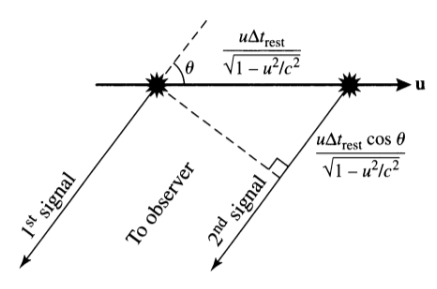
\includegraphics[width=6cm]{chapters/04/dopper}
  \caption{相对论性多普勒频移}
  \label{fig:doppler}
\end{figure}

如图\ref{fig:doppler}所示,由于光源的视向运动的光性差,考虑狭义相对论的时间延缓效应,会导致接受者所观测到的光频发生变化
\begin{equation}
  \upsilon_\mathrm{obs}={\upsilon_\mathrm{rest}\sqrt{1-u^2/c^2}\over 1+v_r/c}
  \label{eq:doppler}
\end{equation}

光源朝向观测者的运动会导致蓝移,远离观测者的运动会导致红移,频移的程度可以用\textbf{红移参数}$z$来描述:
\begin{equation}
  z\equiv{\lambda_\mathrm{obs}-\lambda_\mathrm{rest}\over \lambda_\mathrm{rest}}={\Delta\lambda \over \lambda_{rest}}=\sqrt{{1+v_r/c \over 1-v_r/c}}-1
\end{equation}

相对论效应还会导致在运动坐标系中观测到的速度发生变化:
\begin{align}
  v_x' &={v_x-u \over 1-uv_x/c^2}\\[2mm]
  v_y' &={v_y\sqrt{1-u^2/c^2} \over 1-uv_x/c^2}\\[2mm]
  v_z' &={v_z\sqrt{1-u^2/c^2} \over 1-uv_x/c^2}
\end{align}

由于观测速度的变化主要体现在坐标系运动方向上,因此合速度的方向也会发生变化$\sin\theta={v_y /v}=\gamma^{-1}$,当相对论效应足够强时,$\theta\sim\gamma^{-1}$,即速度会被收束在二倍的$\gamma^{-1}$的张角内,这被称为\textbf{头灯效应(headlight effect)},如图\ref{fig:beaming}所示,同步辐射因此而显现出偏振态

\begin{figure}[hbt]
  \centering
  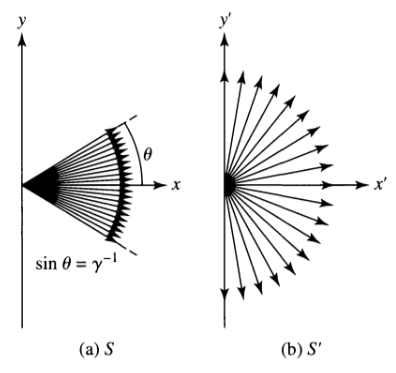
\includegraphics[width=6cm]{chapters/05/beaming}
  \caption{头灯效应}
  \label{fig:beaming}
\end{figure}


\section{相对论动量和能量}
由于要满足相对论性原理,即所有惯性系下动量都应相同,因此定义\textbf{相对论性动量}
\begin{equation}
  \mathbf p=\gamma m \mathbf v
\end{equation}

以及相对论性动能:
\begin{equation}
  K=\underbrace{ \gamma mc^2}_\text{相对论性总能量}-\underbrace{mc^2}_\text{静能量}=mc^2(\gamma-1)
\end{equation}

相对论性总能量还可以写为(作业题):
\begin{equation}
  E^2=p^2c^2+m^2c^4
\end{equation}

该式可适用于计算无质量的粒子,如光子的总能量